\Conclusion

В ходе данной работы была спроектирована и разработана среда для проведения дистанционных испытаний в области защиты информации. Цель данной выпускной квалификационной работы достигнута.

У оргкомитета появилась технологичная и отвечающая всем организационным, техническим и правовым требованиям к проведению мероприятий такого рода автоматизированная система. Модульная архитектура среды позволяет расширять её возможности в будущем, чтобы адаптировать её под новые требования и форматы испытаний, а также учитывать новые запросы как участников, так и организаторов.

Разработанная среда была испытана в условиях реальных соревнований. 2 апреля 2022 города в 10 городах России прошёл заключительный этап школьной олимпиады по защите информации Ugra CTF School 2022. Техническая инфраструктура этапа была основана на разработанной в рамках данной выпускной квалификационной работы среды для проведения испытаний.

\begin{figure}[h!]
  \centering
  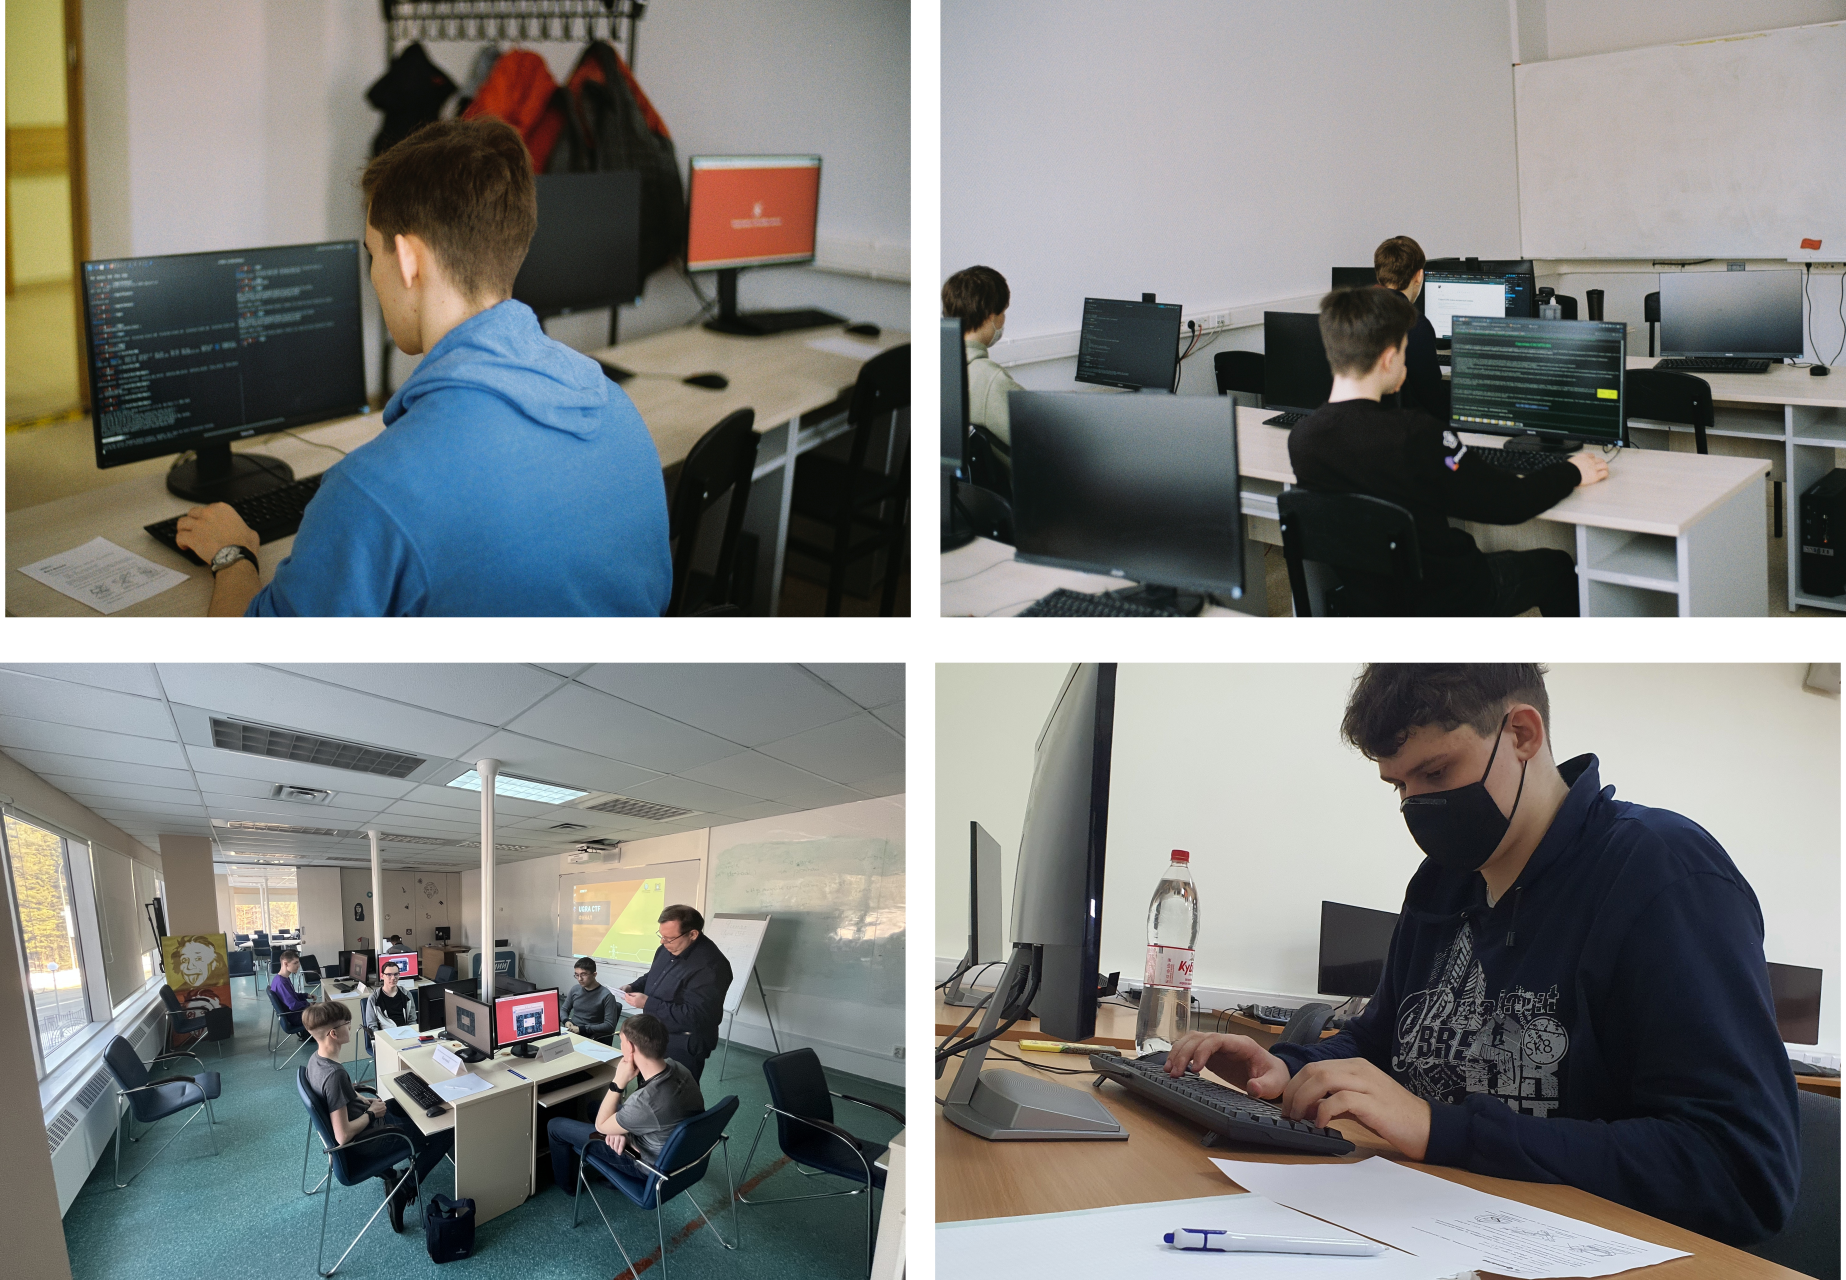
\includegraphics[width=0.9\textwidth]{inc/img/ugractf-22}
  \caption{Ход Ugra CTF School 2022. Верхний ряд: на площадке в Долгопрудном; нижний ряд: в Ханты-Мансийске, Сургуте.}
  \label{fig:Jeopardy}
\end{figure}

Используя личный кабинет в ИС <<Юрт>>, участники могли загрузить произвольный образ гостевой ОС для ВМ VirtualBox до 28 марта. В этот день оргкомитет записал образ на накопители для 56 участников, часть из которых подлежала ручной провизии и замене штатной гостевой ОС Kali Linux на ОС, предоставленную участниками. Накопители были доставлены на площадки представителями оргкомитета лично, либо разосланы почтой.

%% \begin{figure}[h!]
%%   \centering
%%   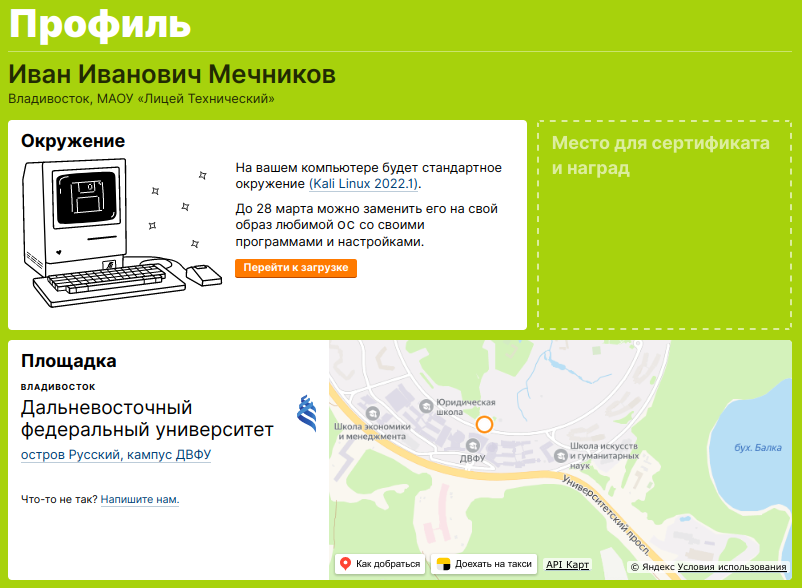
\includegraphics[width=0.8\textwidth]{inc/img/urt-profile}\\
%%   \caption{Профиль участника олимпиады Ugra CTF в ИС <<Юрт>>.} % #
%%   \label{fig:urt-profile}
%% \end{figure}

\begin{figure}[h!]
  \centering
  \includegraphics[width=\textwidth]{inc/svg/downtimes-after}
  \caption{Статистика доступности ресурсов задач с учётом соревнований 2022 года. Данные оргкомитета.}
  \label{fig:downtimes-after}
\end{figure}

Внедрение принципов декларативности и механизмов, автоматизирующих процесс публикации ресурсов игровых задач позволило существенно улучшить их доступность, повысив этот показатель до 99.5\% (рисунок \ref{fig:downtimes-after}). Процесс разработки задач был упрощён благодаря введению абстракций для решения типовых вопросов, наиболее часто возникающих при разработке --- запуску фоновых процессов, выделению адресов и т. п.

Разработанный модуль среды SchoolOS помогла предоставить участникам комфортное окружение для решения задач, отвечающее всем поставленным требованиям, а также упростило организационные процессы: от рассадки участников по местам с помощью индикации на экране до подготовки площадок наблюдателями, освобождёнными от необходимости настраивать компьютеры и устранять возникающие неполадки в болшинстве случаев.

Использование среды позволило обеспечить равные условия участников олимпиады и выявить одно нарушение регламента проведения заключительного этапа олимпиады.
